\chapter{Materiais e Ferramentas}

A descrição dos elementos físicos usados no projeto da lâmpada inteligente pode ser resumida pelo esquema geral do projeto na Figura \ref{esquema}.

\begin{figure}[ht]
    \begin{center}
    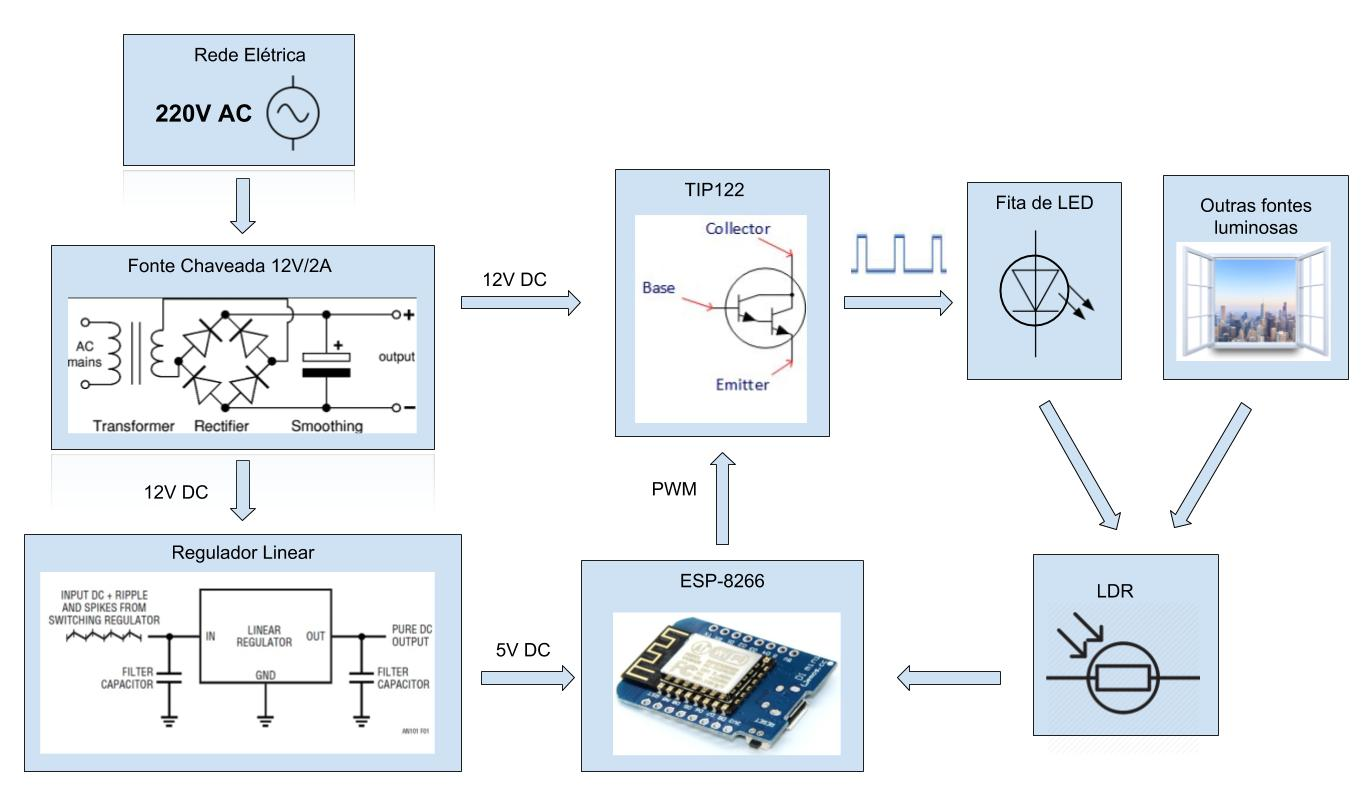
\includegraphics[width=\textwidth]{figuras/esquema_eletrico.jpg}
    \end{center}
    \caption[Esquema geral do projeto da fita de LED MQTT.]{Ilustração do funcionamento do protocolo MQTT com três clientes e o broker trocando mensagens pelo tópico "temperatura".}
    \label{esquema}
\end{figure}

\section{Alimentação}

A fonte de alimentação elétrica do projeto é uma fonte comercial de 12V/1A de padrão comercial “\textit{bivolt}” com plugue P4. Os 12V fornecidos pela fonte serão partilhados pela fonte de iluminação e pelo sistema embarcado. Um regulador baseado no CI AMS1117 será usado para transformar os 12V da fonte em 5V para alimentar o sistema com o microcontrolador. Esse regulador têm sua tensão de saída fixa em 5V e apresenta algumas funcionalidades como limitador interno de corrente e auto-desligamento térmico, e com o arrefecimento adequado ele pode fornecer até 1A que já é mais que o suficiente para o ESP-8266 que consome em torno de 220 mA durante curtos períodos quando está transmitindo via WiFi.

\begin{figure}[ht]
    \begin{center}
    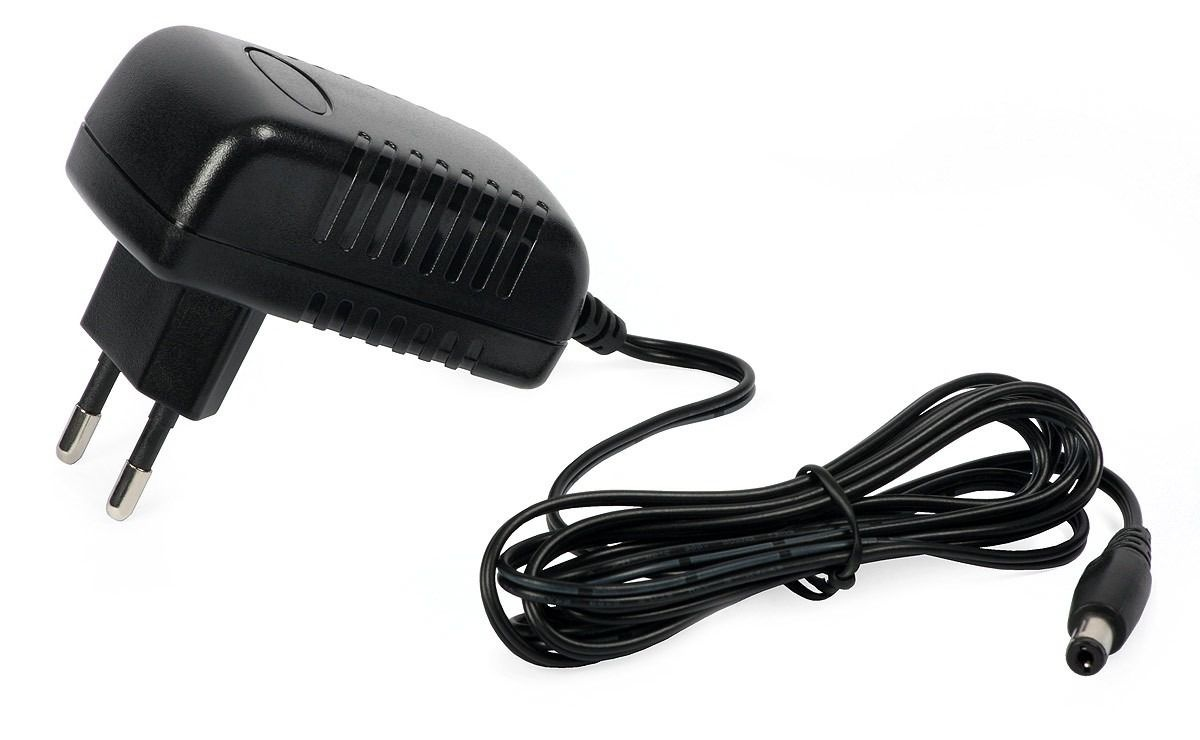
\includegraphics[width=0.5\textwidth]{figuras/fonte.jpg}
    \end{center}
    \caption[Ilustração da fonte chaveada de 12V.]{Ilustração da fonte chaveada de 12V com capacidade de fornecer até 2A.}
    \label{fonte}
\end{figure}

\section{Módulo Microcontrolador}

Como mencionado, o microcontrolador escolhido para o projeto é o ESP-8266 que inclui capacidade de comunicação WiFi. A própria fabricante do CI comercializa alguns módulos que facilitam o desenvolvimento com o ESP-8266 com antenas, LED, memória \textit{flash} e outros periféricos. Um desses módulos, o ESP-12 é usado por diversas empresas para fabricarem seus kits de desenvolvimento com ainda mais facilidades para o desenvolvedor. O kit usado neste projeto é “\textit{Wemos D1 Mini}” que conta com conversor USB-serial, regulador de tensão para transformar os 5V DC provenientes da porta "USB" ou da alimentação externa para os 3.3V DC que o ESP-8266 demanda, oscilador, botão para \textit{reset} e conectores para os pinos de entrada e saída.

\begin{table}
    \centering
    \label{wemos_dados}
    \caption{Especificações do kit \textit{Wemos D1 Mini}}
    \begin{tabular}{ll} 
        \hline
        Kit de desenvolvimento          & Wemos D1 Mini  \\ 
        \hline
        SoC                             & ESP-8266       \\ 
        \hline
        Pinos de I/O digitais           & 11             \\ 
        \hline
        Entradas analógicas             & 1 (3,2V máx)   \\ 
        \hline
        Clock                           & 80 MHz         \\ 
        \hline
        Memória \textit{flash}          & 4 MB           \\
        \hline
    \end{tabular}
\end{table}

O pino de entrada analógica do módulo usado tem uma tensão máxima especificada de 3,2V, apesar de a tensão máxima de entrada do ESP-8266 ser de 1V segundo suas características elétricas \cite{esp}. Isto se deve ao fato de o módulo "\textit{Wemos D1 Mini}" apresentar um divisor de tensão conectado ao pino de entrada analógica do SoC fazendo com que a tensão aplicada a este pino seja mapeada de um intervalo de, 0 a 3,2V no devido pino do módulo, para um intervalo de 0 a 1V no pino do ESP-8266.

\begin{figure}[ht]
    \begin{center}
    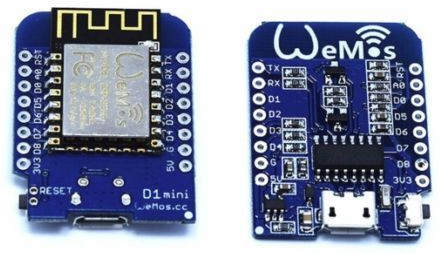
\includegraphics[width=0.4\textwidth]{figuras/wemos.PNG}
    \end{center}
    \caption[Ilustração do módulo \textit{Wemos D1 Mini}.]{Módulo \textit{Wemos D1 Mini} baseado no ESP-8266 visto de cima e de baixo.}
    \label{wemos}
\end{figure}

\section{Sensor de Luminosidade}

O sensor de luminosidade é um "fotoresistor" ou \acf{LDR} cuja resistência, geralmente, diminui com o aumento da intensidade luminosa linearmente. Geralmente são materiais semicondutores de alta resistividade, mas que quando expostos à luz, têm elétrons liberados em sua camada de condução aumentando assim sua condutividade por isso são geralmente chamados de células fotocondutivas. Existem LDRs sensíveis a faixas de radiação ultravioleta, infravermelho e a luz visível, que são os mais comuns.

O LDR usado \cite{ldr} é feito do material semicondutor CdS e apresenta uma curva de resistência em função da intensidade luminosa como mostrada na figura \ref{reta}. Os valores mostrados podem variar um pouco com a temperatura e existe um comportamento transiente quando a luminosidade é variada bruscamente de tempos da ordem de 100ms, o que não se torna relevante para medições menos frequentes que uma repetição por minuto, por exemplo.

\begin{figure}[htp]
    \begin{center}
    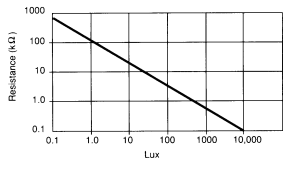
\includegraphics[width=0.4\textwidth]{figuras/reta.PNG}
    \end{center}
    \caption[Gráfico da reisitência \textit{versus} intensidade luminos do LDR.]{Gráfico da reisitência \textit{versus} intensidade luminos do LDR.}
    \label{reta}
\end{figure}

\section{Fita de LED}
A fonte de iluminação é uma fita de LED branca que consiste de elementos de três LEDs e um resistor em série para limitar a corrente, com vários desses elementos ligados em paralelo o que permite que todos os elementos sejam submetidos à mesma tensão e que a fita possa ser cortada em determinados pontos e continue funcionando. A fita de LED adquirida para o projeto tem as especificações listadas na Tabela 3.2.

\begin{figure}[htp]
    \begin{center}
    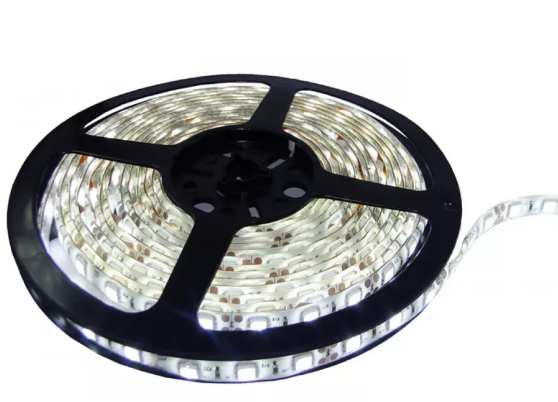
\includegraphics[width=0.3\textwidth]{figuras/fitaled.PNG}
    \end{center}
    \caption[Ilustração da fita de LED branca.]{Ilustração da fita de LED de cor branca fria de 12V.}
    \label{fitaled}
\end{figure}

 

\begin{table}
    \centering
    \label{fitaled_dados}
    \caption{Especificações da fita de LED branca}
    \begin{tabular}{ll} 
        \hline
        Tensão de Operação (V)  & 12            \\ 
        \hline
        Consumo por metro (W/m) & 4.8           \\ 
        \hline
        Comprimento (m)         & 5             \\ 
        \hline
        LEDs por metro          & 60            \\ 
        \hline
        Temperatura da cor (K)  & 6000(frio)    \\
        \hline
    \end{tabular}
\end{table}

O controle da luminosidade será feito por chaveamento da alimentação da fita de LED com \acf{PWM}, técnica que permite controlar digitalmente a potência entregue a atuadores ao determinar a parcela do período em nível lógico alto, de um sinal alternado. O microcontrolador irá chavear um transistor \textit{darlington} “TIP122” \cite{tip122}.

\section{Ferramentas de Desenvolvimento}

\subsection{\textit{Broker} MQTT}

O \textit{broker}, ou servidor, MQTT responsável pelo controle das mensagens intercambiadas na rede será o \textit{broker} da "\textit{Adafruit}" \cite{adafruit}. O serviço oferecido pela \textit{Adafruit} conta com um  \textit{broker} MQTT configurado com níveis de QoS 0 e 1, tópicos especiais como o "\texttt{time/seconds}" que fornece um número de segundos passados desde primeiro de janeiro de 1970 (\textit{Unix Time}) ou o tópico "\texttt{(username)/throttle}" que indica se a limitação de frequência de publicações foi atingida (que na versão grátis do serviço é de 60 vezes por minuto). O seviço da \textit{Adafruit} fornece também uma biblioteca da MQTT própria para \textit{Arduino} que define várias funções de \textit{callback} de subscrições e rotinas de conexão, desconexão e outras.

Uma interface de controle e visualização \textit{web} também é fornecida pela \textit{Adafruit} com possibilidade de implementação de botões, mostradores de valores, gráficos em tempo real, entre outras funcionalidades.

\subsection{Ambiente de Desenvolvimento de \textit{Software}}

O ESP-8266 possui um conjunto de bibliotecas e ferramentas, cujo objetivo é produzir código que, quando compilado, pode ser gravado na memória de programa e executado. Essas ferramentas levam o nome de "SDK" (\textit{Software Development Kit}) e são fornecidas, oficialmente, pela fabricante \textit{Espressif}. Uma comunidade de desenvolvedores do ESP-8266 criou uma estrutura de interfaces e adaptações (\textit{framework}) de código aberto para a SDK oficial para que fosse possível programar com a linguagem "C++" e usar as bibliotecas do \textit{Arduino}.

O desenvolvimento do software foi feito na IDE (\textit{Integrated Development Environment}) "\textit{Visual Studio Code}" da "\textit{Microsoft}" que é essencialmente um editor de texto de código aberto, muitas opções de customização e capacidade de conexão com extensões de terceiros. Uma dessas extensões foi usada, o "PlatformIO", Figura \ref{pio}, que é uma plataforma que conta com compiladores e outras ferramentas de diversos microcontroladores como \textit{Arduino}, ARM, \textit{Atmel} e vários outros. A extensão conta ainda com terminal virtual, monitor de porta serial, ferramentas de depuração de código e suporte à versionamento de código online.

\begin{figure}[ht]
    \begin{center}
    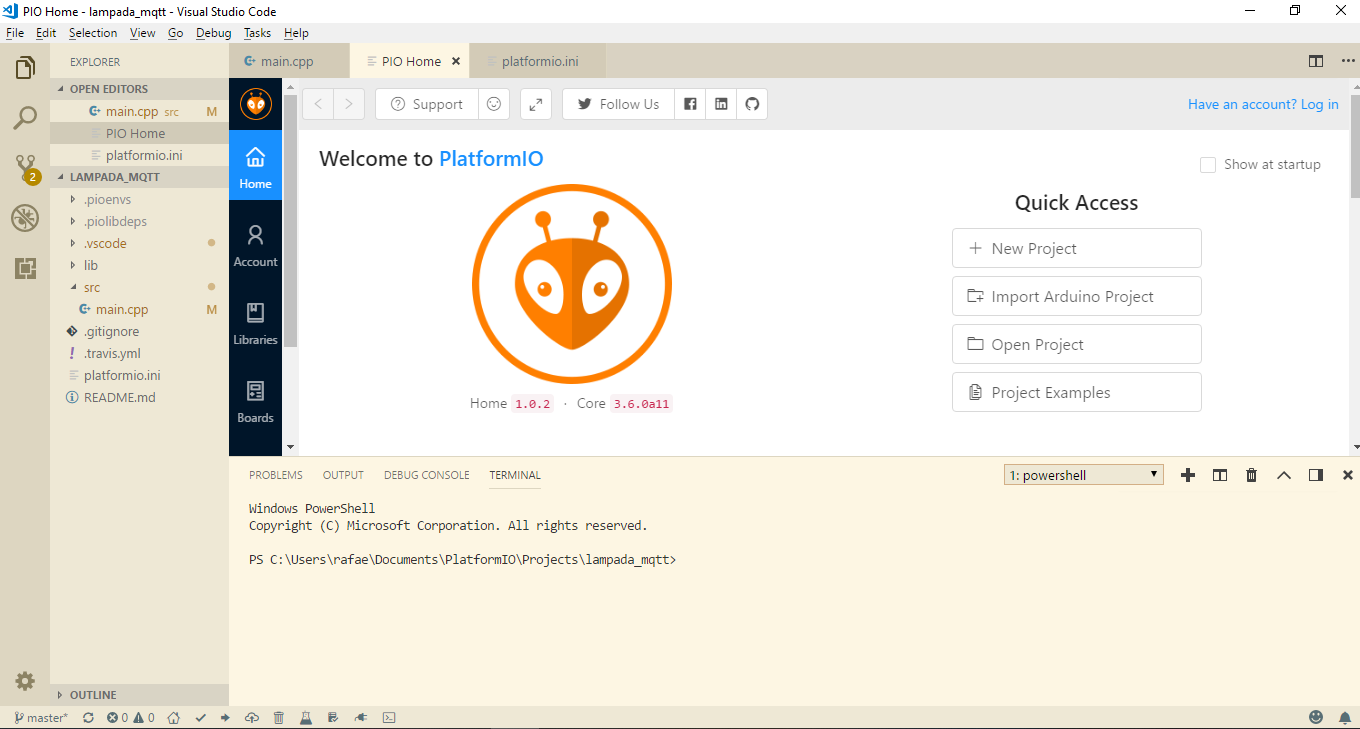
\includegraphics[width=\textwidth]{figuras/pio.PNG}
    \end{center}
    \caption[Ilustração do Visual Studio Code com o PlatformIO.]{Ilustração do ambiente de desenvolvimento "Visual Studio Code" com a extensão "PlatformIO".}
    \label{pio}
\end{figure}

\subsection{Bibliotecas}

Como mencionado, a programação foi feita na linguagem de programação "C++" com algumas bibliotecas de terceiros. A primeira a ser mencionada é a biblioteca do \textit{Arduino} que disponibiliza várias funções e definições que permitem uma grande simplicidade legibilidade do código escrito \cite{arduino}.

Outra biblioteca usada foi "Esp8266WiFi" \cite{espwifi}que disponibiliza várias rotinas relativas a conexão do ESP-8266 como a rede WiFi, reconexão, códigos relativos a camada TCP/IP e outros detalhes importantes para que o uso da internet com o microcontrolador seja possível.

A biblioteca "WiFi \textit{Manager}" \cite{wifimng} foi também usada e permitiu automatizar e generalizar o processo de autenticação do projeto para qualquer rede WiFi por meio da criação de uma página \textit{web} pela qual o usuário pode escolher a rede desejada e informar sua senha para que o ESP-8266 se conecte e salve essas informações em caso de reconexão.
